\paragraph{Measured outcomes.}
All eighteen initial cells completed with valid sealed token/event evidence; no cell was replaced or extended. B1 cells retained 249--314 physical intervals each, with at least 24 per prompt. B4 cells retained 51--64 full-cohort intervals each, with at least 25 per cohort. No eligible interval exceeded the 1.5-second diagnostic cutoff. All-phase API reconciliation includes the preflight and warm-up outputs, while the primary numerator and denominator use timed support only. Cell 16's p021 response ended at EOS after 101 tokens; every other timed response used the 128-token budget. Its eight-prompt coverage remained valid, so this outcome is retained. The artifact reports every cell, per-prompt/cohort support, termination, and exclusions; terminal intervals without a successor have unobserved duration rather than an imputed zero.

Figure~\ref{fig:e1-timing} reports the complete initial campaign. Mean retained-decode rates for native MTP-5, native MTP-11, and cat10 are respectively 13.67, 11.44, and 12.69 tokens/s at B1, and 55.38, 42.15, and 47.28 tokens/s at B4. Cat10 is 7.14\% below MTP-5 at B1 and 14.61\% below it at B4, while exceeding the longer-chain MTP-11 configuration. The paired cat10-minus-MTP-5 differences are $-0.976$ tokens/s at B1 (95\% percentile interval $[-1.085,-0.787]$) and $-8.091$ at B4 ($[-9.680,-5.830]$). Against MTP-11 they are $1.256$ ($[1.157,1.445]$) and $5.133$ ($[4.179,6.811]$). All six contrasts, including MTP-11 minus MTP-5, meet the prespecified precision target; the largest half-width divided by the mean MTP-5 rate is 4.82\%. This does not turn the coarse three-block intervals into evidence of broad workload precision.

\begin{figure*}[t]
\centering
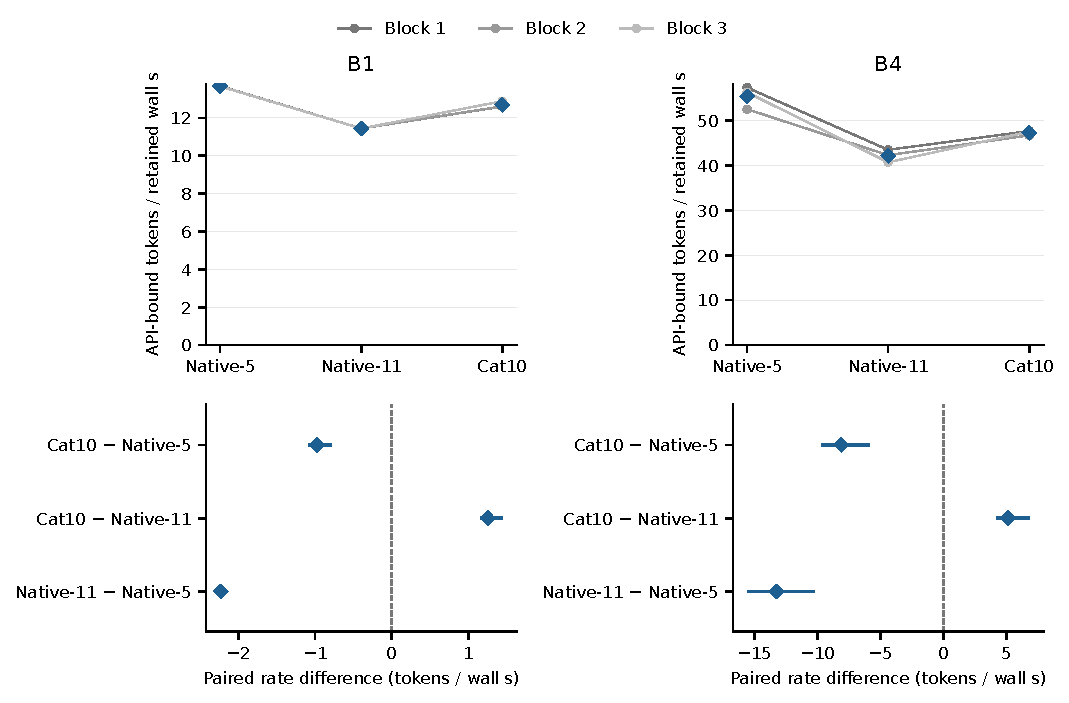
\includegraphics[width=0.94\textwidth]{figures/e1-timing.pdf}
\caption{E1: all eighteen initial fresh-boot cells on the pinned stack. Top: each gray line connects one paired block; blue diamonds mark the mean of three boot rates. Bottom: mean paired differences and the frozen 95\% bootstrap percentile intervals, resampling whole blocks separately at B1 and B4. Rates bind returned API tokens to unique retained wall intervals. These are as-executed instrumented configurations with different attention backends, the disclosed engine-seed deviation, and observed output divergence; they do not isolate a causal tree-algorithm effect.}
\label{fig:e1-timing}
\end{figure*}

\paragraph{Observed continuation divergence.}
A retrospective comparison uses the complete timed API-ID streams, not just rate-support tokens. Across the three pairs of arms, three blocks, two batch conditions, and eight prompts, only 14 of 144 same-block prompt-stream pairs are exactly equal. Comparing the three block pairs within each arm/batch gives 72 equal pairs out of 144. Both native B1 arms repeat exactly in all 24 within-arm comparisons apiece; tree B1 does so in 8/24. At B4 the equality counts are 7/24 for MTP-5, 5/24 for MTP-11, and 4/24 for cat10. These dependent pair counts describe the observed streams, not an estimated population failure probability. They neither identify the source of divergence nor establish full-model sequential equivalence. Together with the seed and backend differences, they limit the result to measured output rates of the tested configurations on fixed input prefixes. No matched-continuation, quality-preservation, or isolated algorithm-speedup claim follows. The retrospective diagnostic does not alter the frozen eligibility, rates, intervals, or precision decisions.
